% CS615 Aspects of System Administration
% Author: Jan Schaumann <jschauma@netmeister.org>
% $Id: slides.tex,v 1.6 2006/03/07 13:55:55 jschauma Exp $

\documentclass[xga]{xdvislides}
\usepackage[landscape]{geometry}
\usepackage{graphics}
\usepackage{graphicx}
\usepackage{colordvi}
\usepackage{fancyvrb}

\fvset{fontfamily=courier,commandchars=\\\{\}}

\begin{document}
\setfontphv

%%% Headers and footers
\lhead{\slidetitle}                               % default:\lhead{\slidetitle}
\chead{CS615 - Aspects of System Administration}% default:\chead{\relax}
\rhead{Slide \thepage}                       % default:\rhead{\sectiontitle}
\lfoot{\Gray{SMTP, HTTP}}% default:\lfoot{\slideauthor}
\cfoot{\relax}                               % default:\cfoot{\relax}
\rfoot{\Gray{\today}}

\newcommand{\smallish}{\fontsize{16}{16}\selectfont}

\vspace*{\fill}
\begin{center}
	\Hugesize
		CS615 - Aspects of System Administration\\ [1em]
		SMTP, HTTP \\ [1em]
	\hspace*{5mm}\blueline\\ [1em]
	\Normalsize
		Department of Computer Science\\
		Stevens Institute of Technology\\
		Jan Schaumann\\
		\verb+jschauma@stevens-tech.edu+
		\verb+http://www.cs.stevens-tech.edu/~jschauma/615/+
\end{center}
\vspace*{\fill}

\subsection{Send me an email!}

\vspace*{\fill}
Start an NetBSD EC2 instance (ami-b618a0de), log in
and send an email from there to {\tt
jschauma@stevens.edu} with a subject line of "CS615 -
SMTP Exercise" using the {\tt mail(1)} command. \\

Be sure to specify your Stevens address as the "From"
address - see the manual page for an example.\\

Review the mail log in /var/log/maillog after sending
your mail.
\vspace*{\fill}

\subsection{Sending...}
\begin{verbatim}
# tcpdump -i xennet0 -w /tmp/t.out port not 22 2>/dev/null &
# mail -s "CS615 - SMTP Exercise" jschauma@stevens.edu -f jschauma@stevens.edu
Hello,

SMTP is simple.

-Jan
.
EOT
# fg
tcpdump -i xennet0 -w /tmp/t.out port not 22 2>/dev/null
^C
\end{verbatim}


\subsection{Sending...}
\begin{verbatim}
# tail -5 /var/log/maillog
Apr  4 15:42:33 ip-10-235-167-232 postfix/pickup[848]: 2A17275438:
        uid=0 from=<jschauma@stevens.edu>
Apr  4 15:42:33 ip-10-235-167-232 postfix/cleanup[765]: 2A17275438:
        message-id=<20160404154233.2A17275438@ip-10-235-167-232.ec2.internal>
Apr  4 15:42:33 ip-10-235-167-232 postfix/qmgr[876]: 2A17275438:
        from=<jschauma@stevens.edu>, size=380, nrcpt=1 (queue active)
Apr  4 15:42:33 ip-10-235-167-232 postfix/smtp[1124]: 2A17275438:
        to=<jschauma@stevens.edu>, relay=spamfilter01.stevens.edu[155.246.14.37]:25,
        delay=0.62, delays=0.04/0.01/0.03/0.54, dsn=2.0.0,
        status=sent (250 Ok: queued as 688CD6F4001)
Apr  4 15:42:33 ip-10-235-167-232 postfix/qmgr[876]: 2A17275438: removed
\end{verbatim}

\subsection{Sending...}
\begin{verbatim}
# tcpdump -t -r /tmp/t.out port 53
IP 10.235.167.232.65498 > 172.16.0.23.domain: 61195+ MX? stevens.edu. (29)
IP 172.16.0.23.domain > 10.235.167.232.65498: 61195 2/0/0
        MX spamfilter01.stevens.edu. 10,
        MX spamfilter02.stevens.edu. 20 (87)
IP 10.235.167.232.65497 > 172.16.0.23.domain: 1949+
        A? spamfilter01.stevens.edu. (42)
IP 172.16.0.23.domain > 10.235.167.232.65497: 1949 1/0/0 A 155.246.14.37 (58)
IP 10.235.167.232.65496 > 172.16.0.23.domain: 39922+
        AAAA? spamfilter01.stevens.edu. (42)
IP 172.16.0.23.domain > 10.235.167.232.65496: 39922 0/1/0 (113)
IP 10.235.167.232.65495 > 172.16.0.23.domain: 26844+
        A? spamfilter02.stevens.edu. (42)
IP 172.16.0.23.domain > 10.235.167.232.65495: 26844 1/0/0 A 155.246.248.24 (58)
IP 10.235.167.232.65494 > 172.16.0.23.domain: 1439+
        AAAA? spamfilter02.stevens.edu. (42)
IP 172.16.0.23.domain > 10.235.167.232.65494: 1439 0/1/0 (113)
\end{verbatim}

\subsection{Sending...}
\begin{verbatim}
# host -t mx stevens.edu
stevens.edu mail is handled by 20 spamfilter02.stevens.edu.
stevens.edu mail is handled by 10 spamfilter01.stevens.edu.
# host spamfilter01.stevens.edu.
spamfilter01.stevens.edu has address 155.246.14.37
# host spamfilter02.stevens.edu.
spamfilter02.stevens.edu has address 155.246.248.24
#
\end{verbatim}

\subsection{Sending...}
\smallish
\begin{verbatim}
# tcpdump -t -r /tmp/t.out port 25
IP 10.235.167.232.65524 > 155.246.14.37.smtp: Flags [S], seq 1528496417,
IP 155.246.14.37.smtp > 10.235.167.232.65524: Flags [S.], seq 3510048077, ack 1528496418
IP 10.235.167.232.65524 > 155.246.14.37.smtp: Flags [.], ack 1, 
IP 155.246.14.37.smtp > 10.235.167.232.65524: Flags [P.], seq 1:72, ack 1, length 71
IP 10.235.167.232.65524 > 155.246.14.37.smtp: Flags [P.], seq 1:38, ack 72, length 37
IP 155.246.14.37.smtp > 10.235.167.232.65524: Flags [.], ack 38, 
IP 155.246.14.37.smtp > 10.235.167.232.65524: Flags [P.], seq 72:244, ack 38, length 172
IP 10.235.167.232.65524 > 155.246.14.37.smtp: Flags [P.], seq 38:119, ack 244, length 81
IP 155.246.14.37.smtp > 10.235.167.232.65524: Flags [P.], seq 244:282, ack 119, length 38
IP 10.235.167.232.65524 > 155.246.14.37.smtp: Flags [.], ack 282,
IP 155.246.14.37.smtp > 10.235.167.232.65524: Flags [P.], seq 282:369, ack 119, length 87
IP 10.235.167.232.65524 > 155.246.14.37.smtp: Flags [P.], seq 119:508, ack 369, length 389
IP 155.246.14.37.smtp > 10.235.167.232.65524: Flags [.], ack 508
IP 155.246.14.37.smtp > 10.235.167.232.65524: Flags [P.], seq 369:400, ack 508, length 31
IP 155.246.14.37.smtp > 10.235.167.232.65524: Flags [FP.], seq 400:499, ack 508, length 99
IP 10.235.167.232.65524 > 155.246.14.37.smtp: Flags [.], ack 500
IP 10.235.167.232.65524 > 155.246.14.37.smtp: Flags [F.], seq 508, ack 500
IP 155.246.14.37.smtp > 10.235.167.232.65524: Flags [.], ack 509
\end{verbatim}
\Normalsize

\subsection{Sending...}
\begin{verbatim}
# tcpdump -t -r /tmp/t.out -X port 25
...
\end{verbatim}

\subsection{Sending...}
\begin{Verbatim}
$ telnet 155.246.14.37 25
Trying 155.246.14.37...
Connected to spamfilter01.stevens.edu.
Escape character is '^]'.
\textbf{220 spamfilter01.stevens.edu ESMTP (fe32969a29a5f461e53bf93b18c8fdb5)}
EHLO ip-10-235-167-232.ec2.internal
\textbf{250-spamfilter01.stevens.edu Hello ec2-54-205-68-41.compute-1.amazonaws.com [54.205.68.41],}
\textbf{        pleased to meet you}
\textbf{250-SIZE 50000000}
\textbf{250-PIPELINING}
\textbf{250-8BITMIME}
\textbf{250 HELP}
MAIL FROM:<jschauma@stevens.edu> SIZE=380
\textbf{250 Sender <jschauma@stevens.edu> OK}
RCPT TO:<jschauma@stevens.edu>
\textbf{250 Recipient <jschauma@stevens.edu> OK}
\end{Verbatim}

\subsection{Sending...}
\begin{Verbatim}
DATA
\textbf{354 Start mail input; end with <CRLF>.<CRLF>}
Received: by ip-10-235-167-232.ec2.internal (Postfix, from userid 0)
        id 2A17275438; Mon,  4 Apr 2016 15:42:33 +0000 (UTC)
To: jschauma@stevens.edu
Subject: CS615 - SMTP Exercise
Message-Id: <20160404154233.2A17275438@ip-10-235-167-232.ec2.internal>
Date: Mon,  4 Apr 2016 15:42:33 +0000 (UTC)
From: jschauma@stevens.edu (Charlie Root)

Hello,

SMTP is simple.

-Jan
.
\textbf{250 Ok: queued as 6A9C76F4004}
\end{Verbatim}

\subsection{SMTP Codes}
SMTP codes consist of three digits in five classes:
\begin{itemize}
	\item {\bf 1xx} --  Mail server has accepted the command, but does not yet
		take any action. A confirmation message is required.
	\item {\bf 2xx} --  Mail server has completed the task successfully
		without errors.
	\item {\bf 3xx} --  Mail server has understood the request, but requires
		further information to complete it.
	\item {\bf 4xx} --  Mail server has encountered a temporary failure. If
		the command is repeated without any change, it might be
		completed. Try again, it may help!
	\item {\bf 5xx} --  Mail server has encountered a fatal error. Your
		request can't be processed.
\end{itemize}

\subsection{Receiving...}
\begin{verbatim}
Date: Mon, 4 Apr 2016 15:42:33 +0000
From: Jan Schaumann <jschauma@stevens.edu>
To: Jan Schaumann <jschauma@stevens.edu>
Subject: CS615 - SMTP Exercise

Hello,

SMTP is simple.

-Jan
\end{verbatim}

\subsection{Receiving...}
\smallish
\begin{verbatim}
From jschauma@stevens.edu  Mon Apr  4 11:42:35 2016
Received: by panix.netmeister.org (Postfix, from userid 1004)
        id 6B0F56513D; Mon,  4 Apr 2016 11:42:35 -0400 (EDT)
Received: from nexus.stevens.edu (nexus.stevens.edu [155.246.14.12])
        by panix.netmeister.org (Postfix) with ESMTP id 2AD596513B
Received: from exchng02.campus.stevens-tech.edu (exchng02.campus.stevens-tech.edu [155.246.14.23])
        by nexus.stevens.edu (Postfix) with ESMTPS id 11E3817F825
Received: from exchng04.campus.stevens-tech.edu (2002:9bf6:f826::9bf6:f826) by
        exchng02.campus.stevens-tech.edu (2002:9bf6:e17::9bf6:e17) with Microsoft
        SMTP Server (TLS) id 15.0.1104.5; Mon, 4 Apr 2016 11:42:34 -0400
Received: from exchng03.campus.stevens-tech.edu (155.246.248.36) by
        exchng04.campus.stevens-tech.edu (155.246.248.39) with Microsoft SMTP Server
        (TLS) id 15.0.1104.5; Mon, 4 Apr 2016 11:42:34 -0400
Received: from exchng03.campus.stevens-tech.edu ([::1]) by
        exchng03.campus.stevens-tech.edu ([fe80::599a:f128:d1b3:4ce7%12]) with
        Microsoft SMTP Server id 15.00.1104.000; Mon, 4 Apr 2016 11:42:34 -0400
From: Jan Schaumann <jschauma@stevens.edu>
To: Jan Schaumann <jschauma@stevens.edu>
Subject: CS615 - SMTP Exercise
Date: Mon, 4 Apr 2016 15:42:33 +0000
Message-ID: <1b1399e9c44b494f99e9d0030f0fa74b@exchng03.campus.stevens-tech.edu>
x-barracuda-apparent-source-ip: 54.205.68.41
x-ms-exchange-parent-message-id: <20160404154233.2A17275438@ip-10-235-167-232.ec2.internal>
Resent-Message-Id: <20160404154235.11E3817F825@nexus.stevens.edu>
\end{verbatim}

\subsection{Receiving...}
\begin{verbatim}
$ tail -f /var/log/maillog
postfix/smtpd[552]: connect from nexus.stevens.edu[155.246.14.12]
postfix/smtpd[552]: 2AD596513B: client=nexus.stevens.edu[155.246.14.12]
postfix/cleanup[6975]: 2AD596513B:
        message-id=<1b1399e9c44b494f99e9d0030f0fa74b@exchng03.campus.stevens-tech.edu>
postfix/cleanup[6975]: 2AD596513B:
        resent-message-id=<20160404154235.11E3817F825@nexus.stevens.edu>
postfix/smtpd[552]: disconnect from nexus.stevens.edu[155.246.14.12]
postfix/qmgr[24644]: 2AD596513B: from=<jschauma@stevens.edu>, size=3116, nrcpt=1 (queue active)
spamd[24829]: spamd: connection from localhost [::1]:58531 to port 783, fd 5
spamd: processing message <1b1399e9c44b494f99e9d0030f0fa74b@exchng03.campus.stevens-tech.edu>
        aka <20160404154235.11E3817F825@nexus.stevens.edu> for spamd:1004
postfix/pipe[8278]: 2AD596513B: to=<jschauma@netmeister.org>, relay=spamassassin, delay=0.29,
        delays=0.05/0.01/0/0.23, dsn=2.0.0, status=sent (delivered via spamassassin service)
postfix/qmgr[24644]: 2AD596513B: removed
postfix/pickup[16387]: 6B0F56513D: uid=1004 from=<jschauma@stevens.edu>
postfix/cleanup[6975]: 6B0F56513D:
        message-id=<1b1399e9c44b494f99e9d0030f0fa74b@exchng03.campus.stevens-tech.edu>
postfix/cleanup[6975]: 6B0F56513D:
        resent-message-id=<20160404154235.11E3817F825@nexus.stevens.edu>
postfix/qmgr[24644]: 6B0F56513D: from=<jschauma@stevens.edu>, size= 3442, nrcpt=1 (queue active)
postfix/local[2264]: 6B0F56513D: to=<jschauma@netmeister.org>, relay=local,
        delay=0.15, delays=0.08/0.01/0/0.06, dsn=2.0.0, status=sent (delivered to command:
        /usr/pkg/bin/procmail)
\end{verbatim}
\Normalsize

\subsection{Receiving...}
\begin{verbatim}
IP 155.246.14.12.37547 > 166.84.7.99.25: Flags [S], seq 2435028943
IP 166.84.7.99.25 > 155.246.14.12.37547: Flags [S.], seq 4137148947, ack 2435028944
IP 155.246.14.12.37547 > 166.84.7.99.25: Flags [.], ack 1
IP 166.84.7.99.51798 > 166.84.67.2.53: 29782+ PTR? 12.14.246.155.in-addr.arpa. (44)
IP 166.84.67.2.53 > 166.84.7.99.51798: 29782 1/2/2 PTR nexus.stevens.edu. (160)
IP 166.84.7.99.51797 > 166.84.67.2.53: 17361+ A? nexus.stevens.edu. (35)
IP 166.84.67.2.53 > 166.84.7.99.51797: 17361 1/3/3 A 155.246.14.12 (173)
\end{verbatim}

\subsection{Receiving...}
\begin{verbatim}
IP 166.84.7.99.25 > 155.246.14.12.37547: Flags [P.], seq 1:41, ack 1
IP 155.246.14.12.37547 > 166.84.7.99.25: Flags [.], ack 41
IP 155.246.14.12.37547 > 166.84.7.99.25: Flags [P.], seq 1:25, ack 41
IP 166.84.7.99.25 > 155.246.14.12.37547: Flags [P.], seq 41:174, ack 25
IP 155.246.14.12.37547 > 166.84.7.99.25: Flags [P.], seq 25:157, ack 174
IP 166.84.7.99.51796 > 166.84.67.2.53: 41349+ MX? stevens.edu. (29)
IP 166.84.67.2.53 > 166.84.7.99.51796: 41349 2/3/5 MX spamfilter02.stevens.edu.
      20, MX spamfilter01.stevens.edu. 10 (241)
IP 166.84.7.99.51795 > 166.84.67.2.53: 51732+ A? nexus.stevens.edu. (35)
IP 166.84.67.2.53 > 166.84.7.99.51795: 51732 1/3/3 A 155.246.14.12 (173)
IP 166.84.7.99.51794 > 166.84.67.2.53: 64776+ A? 12.14.246.155.sbl.spamhaus.org. (48)
IP 166.84.67.2.53 > 166.84.7.99.51794: 64776 NXDomain 0/1/0 (112)
\end{verbatim}


\subsection{Receiving...}
\begin{verbatim}
IP 166.84.7.99.25 > 155.246.14.12.37547: Flags [P.], seq 174:239, ack 157
IP 155.246.14.12.37547 > 166.84.7.99.25: Flags [.], seq 157:1605, ack 239
IP 155.246.14.12.37547 > 166.84.7.99.25: Flags [.], seq 1605:3053, ack 239
IP 155.246.14.12.37547 > 166.84.7.99.25: Flags [P.], seq 3053:3080, ack 239
IP 166.84.7.99.25 > 155.246.14.12.37547: Flags [.], ack 3053, win 4016,
IP 166.84.7.99.25 > 155.246.14.12.37547: Flags [P.], seq 239:290, ack 3080
IP 166.84.7.99.25 > 155.246.14.12.37547: Flags [F.], seq 290, ack 3080
IP 155.246.14.12.37547 > 166.84.7.99.25: Flags [F.], seq 3080, ack 290
IP 166.84.7.99.25 > 155.246.14.12.37547: Flags [.], ack 3081, win 4197
IP 155.246.14.12.37547 > 166.84.7.99.25: Flags [.], ack 291, win 123
\end{verbatim}

\subsection{Receiving...}
\small
\begin{verbatim}
IP 166.84.7.99.50935 > 166.84.67.2.53: 12067 [1au] A? 12.14.246.155.psbl.surriel.com. (59)
IP 166.84.7.99.50935 > 166.84.67.2.53: 39395 [1au] A? 12.14.246.155.bb.barracudacentral.org. (66)
IP 166.84.7.99.50935 > 166.84.67.2.53: 17365 [1au] A? 12.14.246.155.bl.score.senderscore.com. (67)
IP 166.84.7.99.50935 > 166.84.67.2.53: 38635 [1au] TXT? 37.248.246.155.bl.spamcop.net. (58)
IP 166.84.7.99.50935 > 166.84.67.2.53: 10907 [1au] TXT? 21.14.246.155.bl.spamcop.net. (57)
IP 166.84.7.99.50935 > 166.84.67.2.53: 11246 [1au] TXT? 12.14.246.155.bl.spamcop.net. (57)
IP 166.84.67.2.53 > 166.84.7.99.50935: 39395 0/2/7 (206)
IP 166.84.67.2.53 > 166.84.7.99.50935: 12067 0/4/6 (247)
IP 166.84.67.2.53 > 166.84.7.99.50935: 17365 0/4/5 (254)
IP 166.84.67.2.53 > 166.84.7.99.50935: 38635 0/8/9 (354)
IP 166.84.67.2.53 > 166.84.7.99.50935: 13318 0/8/9 (403)
IP 166.84.67.2.53 > 166.84.7.99.50935: 10907 0/8/9 (353)
IP 166.84.7.99.50935 > 166.84.67.2.53: 8582 [1au] A? 37.248.246.155.dnsbl.sorbs.net. (59)
IP 166.84.7.99.50935 > 166.84.67.2.53: 61203 [1au] A? 21.14.246.155.dnsbl.sorbs.net. (58)
IP 166.84.7.99.50935 > 166.84.67.2.53: 59454 [1au] A? 12.14.246.155.dnsbl.sorbs.net. (58)
IP 166.84.7.99.50935 > 166.84.67.2.53: 7289 [1au] A? 12.14.246.155.iadb.isipp.com. (57)
IP 166.84.7.99.50935 > 166.84.67.2.53: 63596 [1au] TXT? 12.14.246.155.sa-trusted.bondedsender.org. (70)
IP 166.84.7.99.50935 > 166.84.67.2.53: 18732 [1au] TXT? 12.14.246.155.sa-accredit.habeas.com.
(65)
IP 166.84.7.99.50935 > 166.84.67.2.53: 43600 [1au] A? 12.14.246.155.bl.mailspike.net. (59)
IP 166.84.67.2.53 > 166.84.7.99.50935: 49122 0/19/80 (1472)
IP 166.84.67.2.53 > 166.84.7.99.50935: 6461 0/6/10 (360)
IP 166.84.67.2.53 > 166.84.7.99.50935: 54452 0/13/14 (607)
IP 166.84.67.2.53 > 166.84.7.99.50935: 8582 0/13/14 (558)
IP 166.84.67.2.53 > 166.84.7.99.50935: 61203 0/13/14 (557)
IP 166.84.67.2.53 > 166.84.7.99.50935: 59454 0/13/14 (557)
IP 166.84.67.2.53 > 166.84.7.99.50935: 7289 0/5/7 (288)
IP 166.84.67.2.53 > 166.84.7.99.50935: 63596 0/18/19 (879)
IP 166.84.67.2.53 > 166.84.7.99.50935: 18732 0/15/16 (742)
IP 166.84.67.2.53 > 166.84.7.99.50935: 43600 0/2/3 (126)
IP 166.84.7.99.50935 > 166.84.67.2.53: 2649 [1au] TXT? nexus.stevens.edu. (46)
IP 166.84.67.2.53 > 166.84.7.99.50935: 2649 0/3/4 (168)
\end{verbatim}
\Normalsize

\subsection{Authenticity}
\begin{verbatim}
$ telnet spamfilter01.stevens.edu 25
Trying 155.246.14.37...
Connected to spamfilter01.stevens.edu.
Escape character is '^]'.
220 spamfilter01.stevens.edu ESMTP (fe32969a29a5f461e53bf93b18c8fdb5)
ehlo localhost
250-spamfilter01.stevens.edu Hello ec2-54-205-68-41.compute-1.amazonaws.com
        [54.205.68.41], pleased to meet you
250-SIZE 50000000
250-PIPELINING
250-8BITMIME
250 HELP
MAIL FROM:<obama@whitehouse.gov>
250 Sender <obama@whitehouse.gov> OK
RCPT TO:<comey@fbi.gov>
550 No such domain at this location
\end{verbatim}

\subsection{Authenticity}
\begin{verbatim}
MAIL FROM:<obama@whitehouse.gov>
250 Sender <obama@whitehouse.gov> OK
RCPT TO:<jschauma@stevens-tech.edu>
250 Recipient <jschauma@stevens-tech.edu> OK
DATA
354 Start mail input; end with <CRLF>.<CRLF>
From: "Barack Obama" <obama@whitehouse.gov>
Subject: Friday

Yo,

Party at my house.
BYOB.

-B
.
250 Ok: queued as 61D4D6F4003
\end{verbatim}

\subsection{Authenticity}
\begin{verbatim}
MAIL FROM:<president@stevens.edu>
250 Sender <president@stevens.edu> OK
RCPT TO:<jschauma@stevens-tech.edu>
250 Recipient <jschauma@stevens-tech.edu> OK
DATA
354 Start mail input; end with <CRLF>.<CRLF>
From: "Barack Obama" <obama@whitehouse.gov>
Subject: Friday

Yo,

Party at my house.
BYOB.

-B
.
250 Ok: queued as 61D4D6F4003
\end{verbatim}

\subsection{Authenticity}
\begin{verbatim}
Date: Mon,  4 Apr 2016 15:35:12 -0400 (EDT)
From: Barack Obama <obama@whitehouse.gov>
To: undisclosed-recipients: ;
Subject: Friday

Yo,

Party at my house.
BYOB.

-B
\end{verbatim}

\subsection{Authenticity}
\begin{verbatim}
From president@stevens.edu  Mon Apr  4 15:35:12 2016                                                
Return-Path: <president@stevens.edu>                                                                
Date: Mon,  4 Apr 2016 15:35:12 -0400 (EDT)
From: Barack Obama <obama@whitehouse.gov>
To: undisclosed-recipients: ;
Subject: Friday

Yo,

Party at my house.
BYOB.

-B
\end{verbatim}

\subsection{SMTP is a Simple Mail Transfer Protocol.}

\begin{itemize}
	\item TCP port 25
	\item DNS MX records
	\item mail may be relayed or processed by many servers in transit
	\item transport is in clear text
	\item SPAM controls may include DNS lookups, bayesian scoring, ...
	\item authenticity not guaranteed
\end{itemize}

\subsection{The Mail System}
Divided into:
\begin{itemize}
	\item {\em Mail User Agent} or MUA, such as {\tt mutt(1)}, {\em Mail.app}, {\em Outlook}, a browser (ugh) ...
	\item {\em Mail Transfer Agent} or MTA, such as {\em postfix},
		{\em sendmail}, {\em qmail}, ...
	\item {\em Mail Delivery Agent} or MDA, such as {\em procmail}
	\item {\em Access Agent} providing access via {\em POP}, {\em IMAP} etc.
\end{itemize}

\subsection{Anatomy of an email message}
An email consists of:
\begin{itemize}
	\item mandatory headers (such as "From ", "Delivered-To: ", ...)
	\item optional headers (such as "From: ", "To: ", "Subject: ", ...)
	\item the (optional) body of the message
\end{itemize}

\subsection{Service Considerations}
\begin{itemize}
	\item outsourcing versus in-house
	\item privacy considerations
	\item spam protections
	\item phishing protections
	\item mail delivery cannons for notifications vs. spam lists
	\item high volume traffic demands fine-tuned systems
	\item high volume traffic implications on logging
\end{itemize}
\vspace{.5in}
See also:
\begin{itemize}
	\item {\tt http://is.gd/JQp1zM}
	\item {\tt http://is.gd/cXyrwX}
	\item {\tt http://is.gd/o6Y5f8}
\end{itemize}

\newpage
\vspace*{\fill}
\begin{center}
    \Hugesize
        Hooray! \\ [1em]
    \hspace*{5mm}
    \blueline\\
    \hspace*{5mm}\\
        5 Minute Break
\end{center}
\vspace*{\fill}

\newpage
\vspace*{\fill}
\begin{center}
	\Hugesize
		Hypertext Transfer Protocol\\ [1em]
	\hspace*{5mm}
	\blueline\\
	\hspace*{5mm}\\
		Today's Universal Internet Pipe
\end{center}
\vspace*{\fill}

%\subsection{Set up an HTTP server.}
%
%\vspace*{\fill}
%Start an EC2 instance and set up an HTTP server to listen on port 8080.
%Add a simple index.html file containing your username.
%
%When done, paste the full URL (ie http:///) into the class IRC channel
%\#cs615asa.
%
%{\tt https://webchat.freenode.net/}
%\vspace*{\fill}

\subsection{HTTP: Hypertext}
\vspace{.5in}
\begin{center}
	\Huge
	W W W
	\\
\vspace{.5in}
	{\em ``The World Wide Web is the only thing I know of whose shortened form
	takes three times longer to say than what it's short for.'' -- Douglas Adams}
\end{center}
\Normalsize


\subsection{HTTP: Hypertext}
\begin{center}
	\includegraphics[scale=0.9]{pics/http-proposal-detail.eps} \\
	\vspace{.5in}
	\verb+http://is.gd/JnZaN6+
\end{center}

\subsection{HTTP}
\vspace{.5in}
\begin{center}
	\Huge
	Hypertext Transfer Protocol
	\\
	\vspace{.5in}
	RFC2616
\end{center}
\Normalsize

\subsection{HTTP}
\vspace{.5in}
\begin{center}
	\Huge
	HTTP is a request/response protocol.
\end{center}
\Normalsize

\subsection{The Hypertext Transfer Protocol}
HTTP is a request/response protocol:
\begin{enumerate}
	\item client sends a request to the server
	\item server responds
\end{enumerate}

\subsection{The Hypertext Transfer Protocol}
HTTP is a request/response protocol:
\begin{enumerate}
	\item client sends a request to the server
		\begin{itemize}
			\item request method
			\item URI
			\item protocol version
			\item request modifiers
			\item client information
		\end{itemize}
	\item server responds
\end{enumerate}

\subsection{HTTP: A client request}
\vspace*{.5in}
\\
\Hugesize
\begin{center}
\begin{verbatim}
$ telnet www.google.com 80
Trying 173.194.75.147...
Connected to www.google.com.
Escape character is '^]'.
GET / HTTP/1.0
\end{verbatim}
\end{center}
\Normalsize
\vspace*{\fill}


\subsection{The Hypertext Transfer Protocol}
HTTP is a request/response protocol:
\begin{enumerate}
	\item client sends a request to the server
		\begin{itemize}
			\item request method
			\item URI
			\item protocol version
			\item request modifiers
			\item client information
		\end{itemize}
	\item server responds
		\begin{itemize}
			\item status line (including success or error code)
			\item server information
			\item entity metainformation
			\item content
		\end{itemize}
\end{enumerate}

\subsection{HTTP: a server response}
%\smallish
\begin{verbatim}
HTTP/1.0 200 OK
Date: Sun, 31 Mar 2013 01:54:40 GMT
Set-Cookie: PREF=ID=c5eb56d629b347cc:FF=0:TM=1364694880:LM=1364694880:
S=sIdRFdxV9YvtQOlG; expires=Tue, 31-Mar-2015 01:54:40 GMT; path=/;
domain=.google.com
Set-Cookie: NID=67=hvBnOob2NoZW4haTJVfajbcyn_jips50lKRe-8nawzdCZ6AukNR
_s8CNHD6ZA-Z2721nA3TpLrNXt-2zyIui23j4kdsdF8Gg--PmGsMOJ3Jv5frEzQG1elHJv92HL-w2;
expires=Mon, 30-Sep-2013 01:54:40 GMT; path=/; domain=.google.com; HttpOnly
Server: gws

<!doctype html><html itemscope="itemscope" itemtype="http://schema.org/WebPage">
<head><meta content="Search the...

\end{verbatim}
%\Normalsize

\subsection{The Hypertext Transfer Protocol}
Server status codes:
\begin{itemize}
	\item {\bf 1xx} -- Informational; Request received, continuing process
	\item {\bf 2xx} -- Success; The action was successfully received,
        understood, and accepted
	\item {\bf 3xx} -- Redirection; Further action must be taken in order to
        complete the request
	\item {\bf 4xx} -- Client Error; The request contains bad syntax or
		cannot be fulfilled
	\item {\bf 5xx} -- Server Error; The server failed to fulfill an
		apparently valid request
\end{itemize}

\subsection{HTTP: A client request}
\smallish
\begin{verbatim}
$ telnet www.cs.stevens.edu 80
Trying 155.246.89.84...
Escape character is '^]'.
GET / HTTP/1.0

HTTP/1.1 302 Found
Date: Sun, 12 Apr 2015 20:37:23 GMT
Server: Apache/2.2.22 (Debian)
Location: http://www.stevens.edu/ses/cs
Vary: Accept-Encoding
Content-Length: 297
Connection: close
Content-Type: text/html; charset=iso-8859-1

<!DOCTYPE HTML PUBLIC "-//IETF//DTD HTML 2.0//EN">
<html><head>
<title>302 Found</title>
</head><body>
<h1>Found</h1>
<p>The document has moved <a href="http://www.stevens.edu/ses/cs">here</a>.</p>
<hr>
<address>Apache/2.2.22 (Debian) Server at www.cs.stevens.edu Port 80</address>
</body></html>
\end{verbatim}
\Normalsize

\subsection{HTTP: A client request}
\smallish
\begin{verbatim}
$ telnet www.stevens.edu 80
Trying 104.16.126.51...
Connected to www.stevens.edu.cdn.cloudflare.net.
Escape character is '^]'.
GET /ses/cs HTTP/1.1
Host: www.stevens.edu

HTTP/1.1 301 Moved Permanently
Date: Mon, 04 Apr 2016 19:55:40 GMT
Content-Type: text/html; charset=iso-8859-1
Transfer-Encoding: chunked
Connection: keep-alive
Location: http://www.stevens.edu/schaefer-school-engineering-science/departments/computer-science
Via: 1.1 varnish
Server: cloudflare-nginx
\end{verbatim}
\Normalsize

\subsection{HTTP: A client request}
\smallish
\begin{verbatim}
$ telnet www.stevens.edu 80
Trying 104.16.125.51...
Connected to www.stevens.edu.cdn.cloudflare.net.
Escape character is '^]'.
GET /schaefer-school-engineering-science/departments/computer-science HTTP/1.1
Host: www.stevens.edu

HTTP/1.1 200 OK
Date: Mon, 04 Apr 2016 19:57:57 GMT
Content-Type: text/html; charset=utf-8
Last-Modified: Mon, 04 Apr 2016 17:40:31 GMT
Via: 1.1 varnish
X-Drupal-Cache: HIT
X-Generator: Drupal 7 (http://drupal.org)
Server: cloudflare-nginx

7c9f
<!DOCTYPE html>
<html lang="en" class="no-js">
<head>
\end{verbatim}
\Normalsize

\subsection{HTTP: A client request}
\begin{center}
	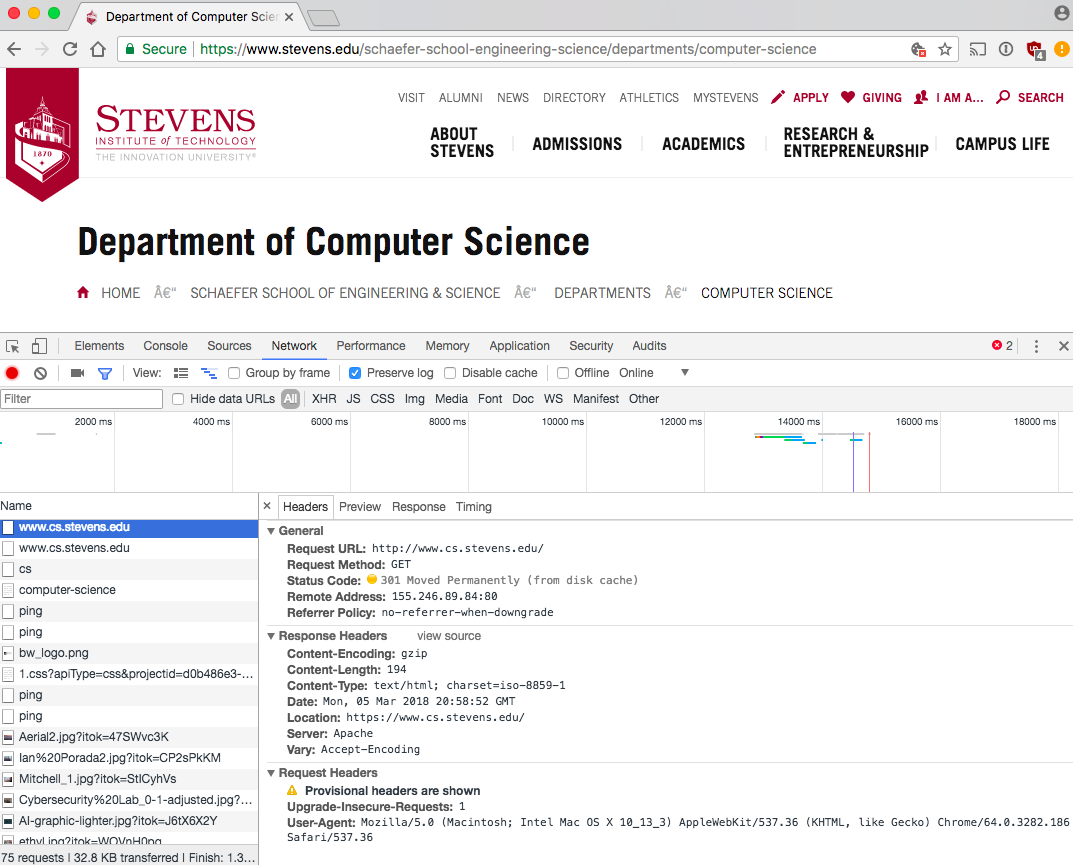
\includegraphics[scale=0.6]{pics/www.cs.stevens.edu.eps}
\end{center}


\subsection{HTTP - more than just text}
HTTP is a {\em Transfer Protocol} -- serving {\em data}, not any specific
text format.

\begin{itemize}
	\item {\tt Accept-Encoding} client header can specify different formats
		such as {\em gzip}, {\em Shared Dictionary Compression over HTTP (SDCH)} etc.
	\item corresponding server headers: {\tt Content-Type} and
		{\tt Content-Encoding}
\end{itemize}
\begin{center}
	
\includegraphics[scale=2.0]{pics/datatransfer.eps}
\end{center}

\subsection{HTTP - more than just static data}
HTTP is a {\em Transfer Protocol} -- what is transferred need not be
static; resources may generate different data to return based on many
variables.

\begin{itemize}
	\item CGI -- resource is {\em executed}, needs to generate
		appropriate response headers
	\item server-side scripting (ASP, PHP, Perl, ...)
	\item client-side scripting (JavaScript/ECMAScript/JScript,...)
	\item applications based on HTTP, using:
		\begin{itemize}
			\item AJAX
			\item RESTful services
			\item JSON, XML, YAML to represent state and
				abstract information
		\end{itemize}
\end{itemize}

%\subsection{HTTPS}
%HTTPS == HTTP over SSL or TLS
%\begin{itemize}
%	\item use of a different server port (443)
%	\item basically use of HTTP protocol just as with plain TCP
%	\item connection initiation:
%		\begin{itemize}
%			\item client initiates a connection to the server
%			\item client sends TLS ClientHello
%			\item client and server perform TLS handshake (according to TLS
%				protocol (RFC 2246))
%			\item client makes regular HTTP requests
%		\end{itemize}
%\end{itemize}
%
%\subsection{Crypto is hard, let's go shopping!}
%Use of SSL has a performance impact:
%\begin{itemize}
%	\item each handshake requires compute-intensive (asymmetric
%		cryptography) certificate
%	\item each session then uses the less intense (symmetric
%		cryptogaphy) session key
%	\item processor-intensive public key encryption algorithms can be
%		offloaded to so-called {\em Crypto Accelerator} cards
%\end{itemize}
%\begin{center}
%	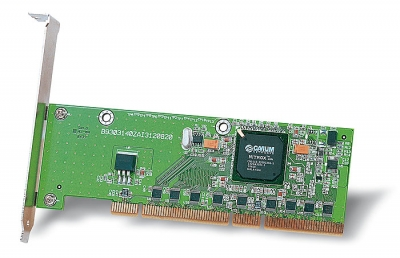
\includegraphics[scale=0.7]{pics/crypto-accelerator.eps}
%\end{center}
%
\subsection{HTTP overload}
Ways to mitigate HTTP overload:

\begin{itemize}
	\item DNS round-robin to many web servers
	\item load balancing
	\item web cache / accelerators (reverse proxies)
	\item content delivery networks
\end{itemize}

These solutions depend on the location within the network and the scale of
the environment.

\subsection{Load Balancing}
\begin{center}
	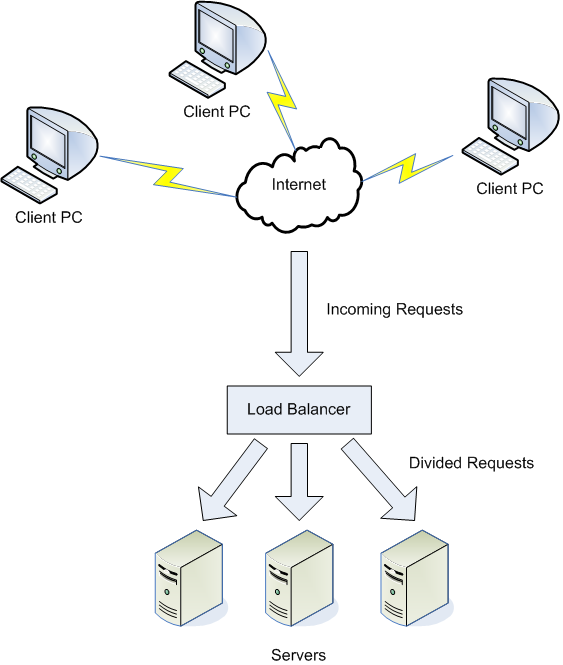
\includegraphics[scale=0.55]{pics/Lb101.eps}
\end{center}

\subsection{Load Balancing: Inbound}
\begin{center}
	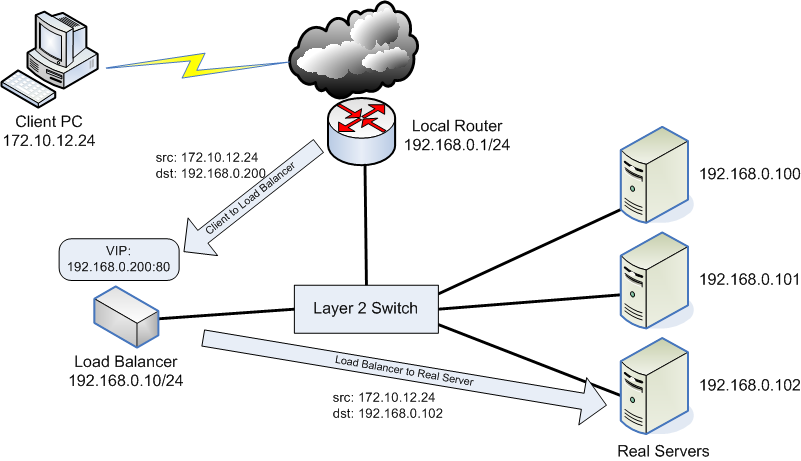
\includegraphics[scale=0.7]{pics/One-armed-inbound.eps}
\end{center}

\subsection{Load Balancing: Outbound}
\begin{center}
	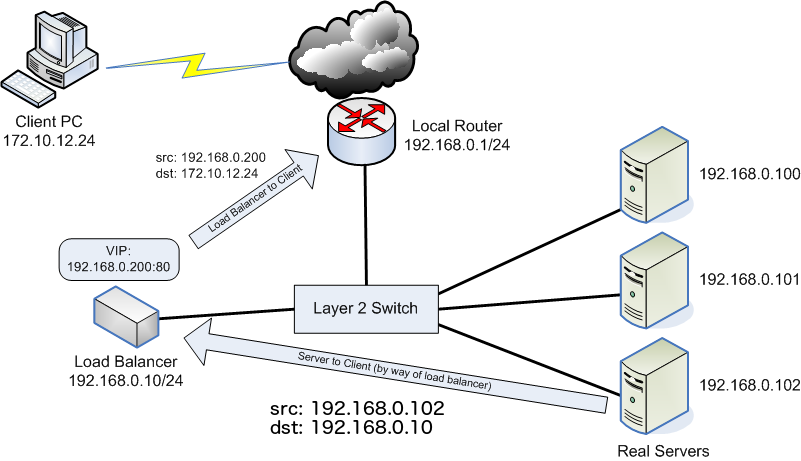
\includegraphics[scale=0.7]{pics/One-armed-outbound.eps}
\end{center}

\subsection{Load Balancing: Direct Server Return}
\begin{center}
	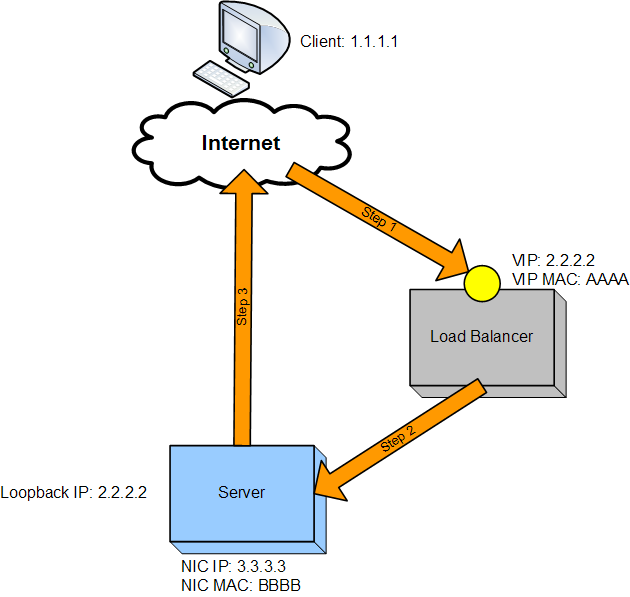
\includegraphics[scale=0.6]{pics/DSR.eps}
\end{center}

\subsection{Content Delivery Networks}
\begin{center}
	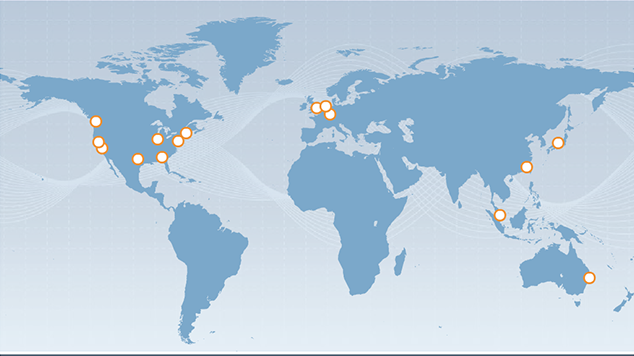
\includegraphics[scale=0.9]{pics/cdn.eps}
\end{center}

\subsection{Content Delivery Networks}
\begin{itemize}
	\item cache content in strategic locations
	\item determine location to serve from via geomapping of IP
		addresses (beware IPv6 aggregation!)
	\item often uses a separate domain to distinguish small
		objects/large objects or dynamic content/static content
	\item either out-sourced or in-house (if your organization is a
		Tier-1 or Tier-2 peering partner)
	\item request routing happens via Global Server Load Balancing,
		DNS-based request routing, anycasting etc.
	\item provides vast amounts of interesting data about your clients
		(see \verb+http://www.akamai.com/stateoftheinternet/+)
\end{itemize}

%\subsection{In-class exercise}
%\vspace{1in}
%\verb+http://www.cs.stevens.edu/~jschauma/615/http-exercise.html+


\subsection{Reading}
SMTP:
\begin{itemize}
	\item \verb+http://bit.ly/5zIadJ+
	\item \verb+http://is.gd/o6Y5f8+
	\item RFC 821, 2821
	\item \verb+aliases(5)+, \verb+mail(1)+
	\item \verb+sendmail(8)+, \verb+postfix(8)+
	\item \verb+https://en.wikipedia.org/wiki/DomainKeys_Identified_Mail+
\end{itemize}

\subsection{Reading}
HTTP etc.:
\begin{itemize}
	\item RFC 2616, 2818, 3875
	\item \verb+http://httpd.apache.org/docs/+
	\item \verb+http://www.w3.org/Protocols/+
	\item REST: \verb+http://is.gd/leSvGa+
	\item CDNs: \verb+http://is.gd/R5DoxA+
		\begin{itemize}
			\item \verb+http://www.edgecast.com/+
			\item \verb+https://aws.amazon.com/cloudfront/+
			\item \verb+http://www.akamai.com/+
			\item \verb+http://www.limelight.com/+
			\item ...
		\end{itemize}
	\item \verb+http://developer.yahoo.com/performance/rules.html+
\end{itemize}



\end{document}
